\documentclass{beamer}

\usepackage{lipsum}
\usepackage[orientation=landscape,size=a0,scale=1.4]{beamerposter}
\usepackage{amsmath,amsthm, amssymb}
\usepackage{setspace}
\usepackage{mleftright}

\usepackage{tikz}
\usetikzlibrary{arrows,shapes,backgrounds} 
\usepackage{tikzpagenodes} 

\tikzset{
	every picture/.style={remember picture},
	na/.style={baseline=-.5ex},
	background grid/.style={draw, black!50,step=.5cm}
}


\setstretch{1}
%\boldmath

%\title[Beamer Poster]{Overleaf example of the beamerposter class}
%\author[welcome@overleaf.com]{Overleaf Team}
%\institute[Overleaf University]
%{The Overleaf institute, Learn faculty}
%\date{\today}

\graphicspath{{images/}}
\usepackage{hyperref}
\hypersetup{
	colorlinks=true,
	linkcolor=blue,
	filecolor=magenta,      
	urlcolor=cyan,
}
%\logo{\includegraphics[height=7.5cm]{example-image-a}}
\usetheme[]{default}

\setbeamertemplate{navigation symbols}{}
\definecolor{main}{HTML}{750f6d}
%\setbeamercolor*{palette primary}{bg=white}
\definecolor{background}{RGB}{250, 250, 250}
\definecolor{cuhk yellow}{RGB}{211, 163, 0}
%\definecolor{alert}{RGB}{}
\setbeamercolor{block title}{bg=main, fg=cuhk yellow}
\setbeamercolor{block body}{bg=main!1!background, fg=black}

\setbeamertemplate{caption}[numbered]
\setbeamercolor{alerted text}{fg=main}

\setbeamertemplate{bibliography item}[text]
\setbeamertemplate{bibliography entry title}{}
\setbeamertemplate{bibliography entry location}{}
\setbeamertemplate{bibliography entry note}{}
\setbeamerfont{bibliography item}{size=\scriptsize}
\setbeamerfont{bibliography entry author}{size=\scriptsize}
\setbeamerfont{bibliography entry title}{size=\scriptsize}
\setbeamerfont{bibliography entry location}{size=\scriptsize}
\setbeamerfont{bibliography entry note}{size=\scriptsize}
%\footlineinfo{123}
%\setbeamercolor{footline}{fg=main, bg=main}  % Disable the page number
\setbeamertemplate{headline}{
	\begin{beamercolorbox}[wd=\paperwidth]{headline}
		\begin{columns}
			\begin{column}{0.125\linewidth}
				\hspace{\fill}
				\centering
				\includegraphics[width=0.85\linewidth]{cuhk-emblem}
			\end{column}
			\begin{column}{0.75\linewidth}
				\vspace{5mm}
				
				\centering\bfseries
				{\fontsize{70}{84}\selectfont Optimal Sensor Fusion using $\mathcal{H}_\infty$ methods} \\ 
				\mdseries
				{\fontsize{60}{72}\selectfont Terrence T.L. Tsang on behalf of the KAGRA Collaboration} \\[5mm]
				{\fontsize{40}{48}\selectfont The Chinese University of Hong Kong. Email: \href{mailto:ttltsang@link.cuhk.edu.hk}{ttltsang@link.cuhk.edu.hk}}
			\end{column}
			\begin{column}{0.125\linewidth}
				\centering
				\includegraphics[width=0.85\linewidth]{KAGRA-logo}
				\hspace{\fill}
			\end{column}
		\end{columns}
	\end{beamercolorbox}
%\color{main!80!background}\rule{\paperwidth}{20pt}
}


\begin{document}
\begin{frame}[t]
%	\begin{abstract}
%		\lipsum[1]
%	\end{abstract}
	\begin{columns}[t]
		
		% Column 1
		\begin{column}{0.32\linewidth}	
			\begin{block}{Introduction: Complementary Filters at KAGRA}
				\begin{itemize}
					\item The pre-isolators of Type-A and Type-B suspensions in KAGRA are equipped with relative sensors and inertial sensors.
					\item A pair of complementary filters (low-pass and high-pass) can be used to combine the sensors into a virtual ``super-sensor'' that has superior noise properties.
					\item In this work, we discuss a scheme that uses $\mathcal{H}_\infty$ methods to synthesize  complementary filters that optimally blend the sensors according to the sensor noises.
				\end{itemize}
					
				\medskip

				\begin{figure}
					\centering
					\includegraphics[width=0.9\linewidth]{suspension_types_transparent.png}
					\caption{Type-A suspensions: input/end test masses, Type-B suspensions: beamsplitter and signal-recycling mirrors, Type-Bp suspensions: power-recycling mirrors, and Type-C suspensions: input/output mode cleaners \cite{Akutsu:2021auw}.}
					\label{fig:suspension_types}
				\end{figure}
			\end{block}
				
			\begin{block}{Methodology: Complementary Filter Problem as an $\mathcal{H}_\infty$ Problem}
				
					$\mathcal{H}_\infty$ method in a nutshell:
					
					\begin{columns}[t, onlytextwidth]
						\begin{column}{0.5\textwidth}
							\begin{enumerate}
								\item As shown in Fig.~\ref{fig:generalized_plant_representation}, define signals $w$, $z$, $u$, and $v$, and hence,
								\item derive a generalized plant $\mathbf{P}(s)$.
								\item $\mathcal{H}_\infty$ synthesis gives an $\mathcal{H}_\infty$ optimal controller $\mathbf{K}_\infty(s)$ that minimizes the $\mathcal{H}_\infty$-norm of the closed-loop plant $\lVert\mathbf{G}(s;\mathbf{K},\mathbf{P})\rVert_\infty$.
							\end{enumerate}
						\end{column}
						\begin{column}{0.5\textwidth}
							\begin{figure}
								\centering
								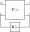
\includegraphics[width=0.5\linewidth]{generalized_plant}
								\caption{Generalized Plant Represenation. }
								\label{fig:generalized_plant_representation}
							\end{figure}
						\end{column}
					\end{columns}
				
					\medskip
					
					\begin{itemize}
						\item The close-loop transfer function $\mathbf{G}(s)$ is defined such that $z=\mathbf{G}(s)w$ and $u=\mathbf{K}(s)v$.
						\item The $\mathcal{H}_\infty$-norm is defined as
						\begin{equation}
							\lVert \mathbf{G}(s) \rVert_\infty = \sup_\omega\bar\sigma \mleft(\mathbf{G}(j\omega)\mright)\,,
						\end{equation}
						where $\bar\sigma$ denotes the maximum singular value and $\omega$ is the angular frequency.
					\end{itemize}

					
		
			
			\end{block}
		\end{column}
		
		% Column 2
		\begin{column}{0.32\linewidth}
			\begin{block}{Methodology: Complementary Filter Problem as an $\mathcal{H}_\infty$ Problem}
%			\begin{columns}[t, onlytextwidth]
%				\begin{column}{0.5\textwidth}
%					\begin{equation}
%						H_1(s) + H_2(s) = 1\,.
%						\label{eqn:complementary}
%					\end{equation}
%				\end{column}
%				\begin{column}{0.45\textwidth}
%					\begin{figure}
%						\centering
%						\includegraphics[width=1\linewidth]{complementary_filter}
%						\caption{Two-sensor complementary filter configuration. $N_1(s), N_2(s)$: sensor noises, $N_\mathrm{super}(s)$: super sensor noise.}
%						\label{fig:two-sensor}
%					\end{figure}
%				\end{column}
%			\end{columns}
%			\medskip
%			
			\textbf{Formulating the complementary filter problem as an $\mathcal{H}_\infty$ problem:}
			
			\medskip
			
			\begin{columns}[t, onlytextwidth]
				
				\begin{tikzpicture}[overlay]
					\node (A) at (0.75\linewidth, -5.5) {};
					\node (B) at (0.75\linewidth, -8.5) {};
					\node (C) at (0.75\linewidth, -12.5) {};
					\node (D) at (0.75\linewidth, -15.5) {};
					\node (E) at (0.75\linewidth, -20) {};
					\node (F) at (0.75\linewidth, -23) {};
					\draw[->,black,line width=2.5mm] (A) -- (B);
					\draw[->,black,line width=2.5mm] (C) -- (D);
					\draw[->,black,line width=2.5mm] (E) -- (F);
					
					\node[align=left] at (0.25\linewidth, -2.5) {Complementary filter configuration: \\ $N_1(s), N_2(s)$: sensor noises,\\ $H_1(s), H_2(s)$: complementary filters,\\ $N_\mathrm{super}(s)$: super sensor noise.};
					\draw[loosely dotted, black, line width=1mm] (0.5\linewidth, -2) -- (0.55\linewidth, -2.3);
					
					\node[draw, align=left] at (0.25\linewidth, -8) {Step 1: \\ Apply constraint $H_1(s) + H_2(s) = 1$.};
					\draw[loosely dotted, black, line width=1mm] (0.52\linewidth, -7.5) -- (0.7\linewidth, -7);
					
					\node[draw, align=left] at (0.25\linewidth, -13) {Step 2: \\ Model the sensor noises with \\ transfer functions $\hat{N}_1(s)$ and $\hat{N}_2(s)$.};
					\draw[loosely dotted, black, line width=1mm] (0.52\linewidth, -13) -- (0.7\linewidth, -14);
					
					\node[align=left] at (0.25\linewidth, -18.25) {$\Phi_1$ and $\Phi_2$ are white noises \\ that has power spectrum \\ with unitary amplitude.};
					\draw[loosely dotted, black, line width=1mm] (0.43\linewidth, -18.25) -- (0.48\linewidth, -17.75);
					
					\node[draw, align=left] at (0.25\linewidth, -24.5) {Step 3: \\ Add weighting functions $W_1(s)$  \\ and $W_2(s)$. \\ Define the generalized plant $\mathbf{P(s)}$ \\ as Eqn.~\ref{eqn:generalized_plant_complementary_filter}.};
					\draw[loosely dotted, black, line width=1mm] (0.5\linewidth, -23) -- (0.7\linewidth, -21.5);
					
					\node[align=left] at (0.25\linewidth, -31.5) {$W_1(s)$ and $W_2(s)$ are the \\ inverse of the frequency dependent \\ specification of the sensor noises.};
					\draw[loosely dotted, black, line width=1mm] (0.43\linewidth, -30.5) -- (0.5\linewidth, -30);
					
					\node[draw, align=left] at (0.25\linewidth, -36) {Finally: \\ $\mathcal{H}_\infty$ synthesis gives optimal $H_1(s)$.} ;
				\end{tikzpicture}
				\begin{column}{0.45\textwidth}

				\end{column}
			\begin{column}{0.5\textwidth}
					\begin{figure}[!h]
					\centering
					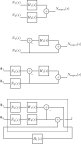
\includegraphics[width=1\linewidth]{from_complementary_filter_to_generalized_plant}
					\caption{From a simple complementary filter configuration to generalized plant representation.}
					\label{fig:from_complementary_filter_to_generalized_plant}
					\end{figure}
				\end{column}
			\end{columns}
			
			\medskip
			
			The generalized plant is given by
			\begin{equation}
				\mathbf{P}(s) = 
				\begin{bmatrix}
					0 & \hat{N}_2(s) W_2(s) & 1 \\
					\hat{N}_1(s) W_1(s) & -\hat{N}_2(s) W_2(s) & 0 \\
				\end{bmatrix}\,.
				\label{eqn:generalized_plant_complementary_filter}
			\end{equation}
			If we set $W_1(s)=1/\hat{N}_2(s)$ and $W_2(s)=1/\hat{N}_1(s)$, then
			\begin{equation}
				\lVert \mathbf{G}(s) \rVert_\infty \approx 
				\begin{cases}
					\sup_\omega \lvert \frac{N_\mathrm{super}(j\omega)}{\hat{N}_2(j\omega)} \rvert \,, & \lvert N_\mathrm{super}(j\omega) \rvert \gg \lvert \hat{N}_2(j\omega) \rvert\,,\\
					\sup_\omega \lvert \frac{N_\mathrm{super}(j\omega)}{\hat{N}_1(j\omega)} \rvert\,, & \lvert N_\mathrm{super}(j\omega) \rvert \gg \lvert \hat{N}_1(j\omega) \rvert\,.
				\end{cases}
				\label{eqn:closed_loop_plant_complementary_filter}
			\end{equation}
			Minimizing $\lVert \mathbf{G}(s) \rVert_\infty$ is approximately equal to minimizing a cost function
			\begin{equation}
				J = \sup_\omega\mleft(\log \lvert N_\mathrm{super}(j\omega)\rvert-\log\min(\lvert N_1(j\omega) \rvert, \lvert N_2(j\omega)\rvert)\mright)\,,
			\end{equation}
			where is the maximum difference between the log super sensor noise and the lower bound of the sensor noises.
			\end{block}
			
			\begin{block}{Results: Synthesizing Complementary Filters for SRM in KAGRA}
				\begin{columns}[t, onlytextwidth]
					\begin{column}{0.55\textwidth}
						1
					\end{column}
					\begin{column}{0.45\textwidth}
						\begin{figure}
							\centering
							\includegraphics[width=1\linewidth]{noise_fit}
							\caption{Sensing noises of the SRM preisolator sensors.}

							\label{fig:noise_fit}
						\end{figure}
					\end{column}
				\end{columns}
				
				\begin{columns}[onlytextwidth]
					\begin{column}{0.5\textwidth}
						\begin{figure}
							\centering
							\includegraphics[width=1\linewidth]{complementary_filters_hinfinity}
							\caption{Filters synthesized using $\mathcal{H}_\infty$ method.}
							\label{fig:complementary_filters_hinfinity}
						\end{figure}
					\end{column}
					\begin{column}{0.5\textwidth}
						\begin{figure}
							\centering
							\includegraphics[width=1\linewidth]{super_sensor_noise_tf}
							\caption{Predicted super sensor noise}
							\label{fig:super_sensor_noise_tf}
						\end{figure}
					\end{column}
				\end{columns}
			\end{block}

		\end{column}
	
		% Column 3
		\begin{column}{0.32\linewidth}
			\begin{block}{Results: Synthesizing Complementary Filters for SRM in KAGRA (Cont.)}
			
			\begin{columns}[onlytextwidth]
				\begin{column}{0.45\textwidth}
					1
				\end{column}
				\begin{column}{0.5\textwidth}
					\begin{figure}
						\centering
						\includegraphics[width=1\linewidth]{super_sensor_noise_comparison}
						\caption{Comparison between the super sensor noises predicted using filter design from \cite{Sekiguchi:2016bmv, vanHeijningen:2018cpc} and the proposed method.}
						\label{fig:super_sensor_noise_comparison}
					\end{figure}
				\end{column}
			\end{columns}

			\medskip
			
			\begin{table}
				\begin{tabular}{|c|c|c|c|}
					\hline
					& RMS ($\mu\text{m}$) & RMS (0.1-0.5 Hz) ($\mu\text{m}$)& ASD (10 Hz) ($\mu\text{m}/\sqrt{\text{Hz}}$)\\
					\hline
					$N_\text{super, 1}$ & 0.5895 & 0.2400 & 4.443e-6\\
					\hline
					$N_\text{super, 2}$ & 0.4726 & 0.1650 & 4.443e-6\\
					\hline
					$N_{\text{super}, \mathcal{H}_\infty}$ & 0.3631 & 0.1041 & 2.087e-5\\
					\hline
					Lower bound & 0.0462 & 0.01422 & 4.443e-6\\
					\hline
				\end{tabular}
				\caption{RMS, band-limited RMS, and ASD values at 10 Hz of the super sensor noises predicted using filter design from \cite{Sekiguchi:2016bmv,vanHeijningen:2018cpc} and the proposed method (\textbf{lower the better}).}
				\label{table:metrics}
			\end{table}

			\end{block}
			\begin{block}{Conclusion}
				\begin{itemize}
					\item The complementary filter problem is formulated as an $\mathcal{H}_\infty$ optimization problem.
					\item Complementary filters can be synthesized using $\mathcal{H}_\infty$ method with no information other than the sensing noises themselves.
					\item The method is exemplified using SRM preisolator sensors and is shown to able to generate filters that better reduce the RMS of the super sensor noise especially around the microseism band.
					\item While the $\mathcal{H}_\infty$ filters perform worse at 10 Hz, 3 orders of magnitude reduction in super sensor noise ASD (compared to LVDT) can still be achieved.
				\end{itemize}
			\end{block}
			\begin{block}{References}
				\bibliographystyle{unsrt}
				\bibliography{poster_terrence_tak_lun_tsang}
			\end{block}
		\end{column}
	\end{columns}
\end{frame}
\end{document}
